\graphicspath{ {./Chapitre1/} }

\chapter{Generation de terrain sémantique}
\minitoc
\teaser{
	 \includegraphics[width=0.9\linewidth]{Figures/Render/figureTeaser.png}
	 \centering
	  \caption{Our method can produce different scenes including coral islands and canyons at multi-scale using environmental objects to represent terrain features.}
	\label{EnvironmentObjects-fig:teaser}
	}

\section{Introduction}
\label{EnvironmentObjects-sec:introduction}
Automated terrain generation is a key component of natural scene digital modeling for animated movies and video games. Many landscapes have been studied and are synthesised with more and more realism. 
Different processes can be used and combined to achieve these scenes: fractal terrains \cite{Musgrave1989,Prusinkiewicz1993a}, erosion simulation \cite{Cordonnier2023, Mei2007}, manual modeling \cite{DeCarpentier, Guerin2022}, geological simulation \cite{Cortial2019,Cordonnier2017a}, ... The high quality of synthesis for such environment is due to the possibility to observe these environments from many point of views: long-distance gazing, hiking on mountains, remote sensing, aerial imaging, ... 
Thanks to the quality of the digital modeling, the entertainment industry display often breathtaking land scenes.

Underwater scenes are rarely created in these media for multiple reasons: these environments are not completely understood and mastered as much as land environments because they are difficult to access, we lack the capacity to see them at a larger scale (unlike mountains for example) and the underlying process that forms these landscapes are much more complex to simulate.

These limitations cause animated movies and video games studios to avoid as much as possible underwater environments. 

However, these environments are important for the study of biology, geology, and, by extension, robotics. Due to the complexity, limitations and danger of underwater human operations, underwater robots are more and more used for marine environment monitoring\cite{Maslin2021, Williams2016, Dunbabin2020, Palmer2021}. Yet the validation process of such underwater robot is expensive, with heavy logistic, and it is often  impossible to find the appropriated environment to test the system. Thus, underwater robotics requires simulation capacities, to be able to test the robot's algorithms in very specific environment and conditions. But for now, roboticians are lacking the capacity to test on realistic virtual scenes, and so only test them on synthetic scenarios that do not correlate with real world terrains. For that, they need to manipulate more precisely the characteristics of the underwater environment, at different scales.

The difficulties to visualize and study the underwater environments on a large scale at the same time as a small scale is an obstacle to the procedural generation and simulation of scenes that are coherent in these two different scales. 
A solution to this problem could be a bottom-up approach, simulating at the smallest scale the behaviour of all the elements of the environment. Computing such a simulation in order to generate an entire ecosystem is an near-impossible task due to time and memory complexity. 

The method we propose provides a way to procedurally generate environments on multiple scales without introducing such complexity by using a sparse representation of the environment using environmental objects.
The environmental objects only have access to local values of the environments to spawn, grow and die. The use of local interaction with environment values removes the need for complex interconnections between all elements of the terrain, providing a parallelisable generation process at large to small scales.
Defining environmental objects of the terrain as parametric models based on point, curve or region skeletons provides a lightweight representation of the terrain that the user can interact with. The interaction with the simulation process is still a difficult task \cite{Smelik2014}.
Our method does not aim for a visually realistic generation, but for a plausible terrain depending on geological and biological constraints, guided by the user. Using state of the art modeling of the geometry of the environmental objects of the terrain could achieve realistic results. We illustrate the method through the generation of coral islands and reefs.

Our main contribution are the introduction of a sparse representation of the terrain elements as environmental objects, the use of fitting functions to incorporate biological rules in the simulation process avoiding physic simulation and an interactive simulation based on geological events for underwater landscapes.


\section{Related works}
\label{EnvironmentObjects-sec:related-works}
Procedural terrain generation has been heavily studied for the last 40 years \cite{Galin2019}. Researches in this topic try to find new solutions to compromise between realism, user control and efficiency \cite{Gain2009}. Using fractal noise parametrized to resemble real landscape has been an important first step \cite{Musgrave1989} as it's a fast and light solution to generate procedurally the appearance of mountains. The lack of user control pushed newer works toward the use of controlled noise by including real DEM in the process through learning \cite{Kapp2020, Brosz2007}, while the rise of deep learning technologies gave higher control to the user through sketches \cite{Guerin2017, Talgorn2018}. \\
By including expert knowledge of tectonic process and subsurface geology, some algorithms tend to get more realistic \cite{Patel2021, Cortial2019, Michel2016}. \\
While these algorithms are able to generate large-scale landscapes, the finer details of the terrain is often computed by the use of erosion simulation \cite{Cordonnier2023, Schott2023, Paris2019}. This process can be expensive in time but results in more plausible surfaces.

All the algorithms aim to reproduce plausible relief in terrestrial landscapes, mostly limited to alpine landscapes, but a lack of research can be found in almost all other biomes. Underwater landscapes generation, for example, has been almost completely absent from literature for many reasons: the difficulty of accessing the area, the lack of visibility under water and the complex physics of underwater geology and biology make the algorithms adapted for this environment scarce. \\
The majority of the ocean floor can be represented as a fractal terrain \cite{Mareschal1989}. While stochastic noise can be sufficient to model the ocean floor, this process won't cover areas with the biggest biomass, near shallower waters such as near coasts and islands. \\
Due to the impossibility to observe the large-scale and the small-scale of underwater environments, some works related to geology model large structures like the profile shape of the coral reef \cite{Bosscher1992}, simulate its surface growth \cite{Li2021}, or use procedural algorithms for single polyp \cite{Abela2015}. We however don't have a mix of the different scales, and neither methods take into account the environment such as the topography or the interaction of different terrain elements. This is mainly due to the fact that the evolution time for each scale varies from a span of weeks to thousands of years.

In an ecosystem, any element of the system has an impact on their surrounding. Simulating each physical properties such as shading, heat, humidity may require enormous computation power. By considering these properties as scalar fields surrounding the whole scene, and that elements of the terrain affect locally the scalar fields, we can simplify the computation of the physical properties of the environment \cite{Grosbellet2016, Guerin2016a}. This process provides a scalable system from which scene details are rendered in a plausible way. In a similar way, other works represent the wind flow as a composition of local vector fields \cite{Wejchert1991}, avoiding complex fluid simulation while providing user control in a lightweight model. We extend these works by incorporating a time-evolution system such that the scene can be dynamic.


\section{Method}
\label{EnvironmentObjects-sec:method}
The overall pipeline of the method is based on simple incremental generation like most rule-based systems. In this type of system, the final state is defined either by reaching equilibrium, or by verifying specific conditions, such as a maximum number of iterations. 
We define our pipeline in three phases (Figure~\ref{EnvironmentalObjects-fig:pipeline}): the initialization phase that describe the generation and simulation rules, the iterative phase generating populating the terrain with our environmental objects and finally the output.


\subsection{Pipeline overview}
\label{EnvironmentObjects-sec:pipeline}

\begin{figure*}
    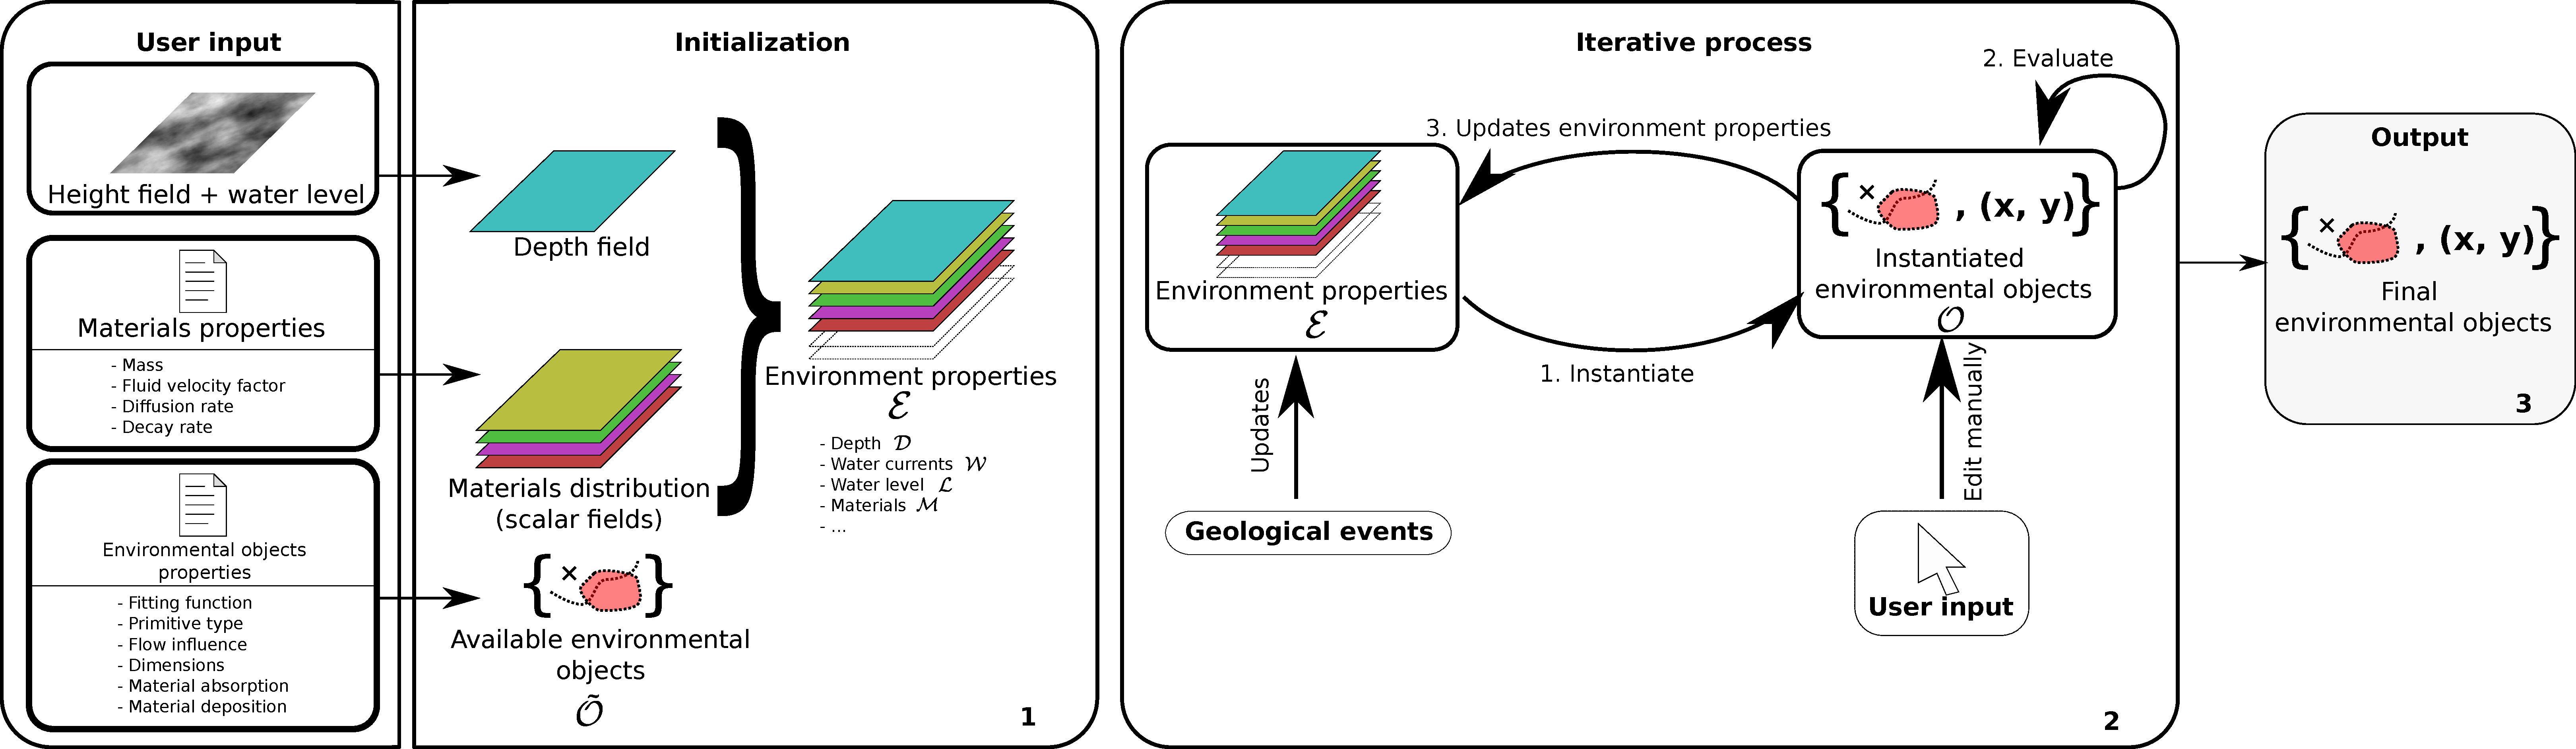
\includegraphics{Figures/pipeline.pdf}
    \caption{Overview of the pipeline of the method. The user provides as input an initial height field and sets the water level, as well as a definition of the materials properties and environmental objects properties that will be used in the iterative process. These inputs are initialized as an initial set of environmental objects and scalar fields that represents the environment values. In the iterative loop, new environmental objects are instantiated using the current state of the environment at their optimal position. The existing environmental objects in the terrain reevaluate their fitting function to grow or die and update the environment values locally. At each iteration, geological events can update the environment values, while the user can interact directly with the environmental objects. The result of the whole process is a set of environmental objects which is a sparse representation of the elements of the scene. }
    \label{EnvironmentalObjects-fig:pipeline}
\end{figure*}

The generation of the terrain is initialized using an initial height field $\height$ and a water level $\Wlevel$. The height field provides variation on the depth $\depth$, which can influence the generation process of the scene. We set $\depth = \height - \Wlevel$. \\
The list of available environmental objects $\availableObjects$, representing the different elements that can be present in the scene, are provided with their properties: type, size, generation rules, growing conditions and effects on the environment values (Section~\ref{EnvironmentObjects-sec:environmental-objects}). \\
Finally, different materials can be defined with their properties such as diffusion speed, mass, damping factor and influence from the water currents. Materials distributions are represented as a scalar field $\material: \R^2 \to \R$ and water currents as a vector field $\Water: \R^2 \to \R^2$ that can be evaluated by the environmental objects of the scene to simulate their growth and spawn at the most probable position. The environmental properties $\environment = (\depth, \Water, \Wlevel, \material)$ is composed of depth, water currents, water level and materials distribution information at any point of the terrain (Section~\ref{EnvironmentObjects-sec:communication}). \\
The definition of environmental objects' properties and environment properties is done with field experts, providing the pertinent parameters required to model the evolution of the terrain elements using expert knowledge (Section~\ref{EnvironmentObjects-sec:biology}). Additional properties can easily be added to the environment properties $\environment$ in order to fit to the experts needs, such as atmospheric pressure, humidity, temperature, ... \\
The generation phase can optionally be started with an initial set of environmental objects present in the scene. 

%- Main loop \\
Once the initialization phase is done, the generation begins. The generation process is incremental and its main loop is composed of two different steps: the instantiation of new environmental objects then the update of the environment.
% - Object instantiation \\
At each iteration, new environmental objects can be created at their most fitting locations if possible. The generation rules provided in the initialization phase are used to find the optimal position from stochastic sampling (Section~\ref{EnvironmentObjects-sec:generation-rules}). 
All environmental objects are evaluating their state analytically using the fitting function provided as input (Section~\ref{EnvironmentObjects-sec:obj-evaluation}).
% Once the new objects are instantiated, the process can continue.
% - Environment update \\
Once the instantiation step is done, the environment's values are updated by each environmental object by deposing and absorbing some of the available materials (Section~\ref{EnvironmentObjects-sec:materials}) while modifying the water currents (Section~\ref{EnvironmentObjects-sec:water-currents}) around them. Finally, water currents and height field's gradient displace materials of the terrain at each iteration.
% We consider the water currents to be a steady-state flow, allowing us to remove the variation from time in the flow equations.
% The water currents are updated locally by each environmental object using an analytical form $W^*(\p) = W(\p) + \omega(\p)$.
During the generation process, the user can alter directly the distribution and shapes of the environmental objects (Section~\ref{EnvironmentObjects-sec:manual-interaction}) and perturb the generation process by planning geological events that have impacts on the environment values (Section~\ref{EnvironmentObjects-sec:events}).

% - Output result \\
The output of our system is a set of environmental objects disposed in the plane. We do not provide the 3D representation of the environmental objects, letting the user define the rendering method. The figures used in the paper use a mix of implicit surfaces and triangular meshes.



\subsection{Environmental objects}
\label{EnvironmentObjects-sec:environmental-objects}

Environmental objects are rule-based objects following rules depending on their local environment for evaluation their state in their life cycle. We can see them as a life form in the way that they are created and eroded with time. During their lifetime, they influence their local environment by depositing and absorbing materials around them and influencing the water currents. The environment objects are described spatially as a single point, a parametric curve or a region.

% \subsubsection{Object's life cycle}
We consider that all environmental objects follow a life cycle of spawning, growing and dying. While many environmental objects of a terrain is not a living being, we assume that evolution of relief, for example, starts at one point in time, grow as the geological factors force it to and is eroded until a point where this environmental object can not be distinguished from the rest of the environment. 

Environmental objects are spawn stochastically in the terrain at the optimal fitting position. This position is determined from a generation rule given by the user for each of the environmental objects, which is dependant on the environment state.
Once the environmental object is present in the scene, it will continuously evaluate its fitting function to determine its state in the life cycle. If the evaluation results as less than zero, the environmental object dies and it is removed from the list of environmental objects present in the scene. While the environmental object remains, it will continue influencing its environment, by absorbing and depositing material around it and by influencing the water currents. 

\subsubsection{Generation rules}
\label{EnvironmentObjects-sec:generation-rules}
Generation rules provides, for each environmental object, a fitting function $\fittingFuncObj$ defining the most probable location for an environmental object to spawn. Fitting functions' parameters contains, for every point $\p$, the environmental values $\environment_p$ (the amount of each material available $\material(\p)$ and the velocity and direction of the water currents $\Water(\p)$) and information about surrounding environmental objects $\objects$ (signed distance from the closest punctual environmental object or curve defining curve- and region-based environmental objects, curvature of the curve, and start and end points of the curve-based environmental objects).

% \subsubsection{Point, curve and region generation}
The seed point of a spawning environmental object is defined by a stochastic sampling of the plane. We propose different optimization means to find the optimal fitting position, depending on the environmental object shape.

The spawning position of a punctual environmental object is found at the local maxima of the fitting function from a seed point. The optimisation process simply follows the field's gradient $\nabla \fittingFuncObj$ until the local maxima is reached.

A region is defined as an isocontour of the field for which the target area $\Area$ is found. From the seed point, we follow the isolevel of the fitting function $\nabla \fittingFuncObj^\perp$ until a loop is created to define the initial condition of the shape. Using the Active Contours algorithm, we can optimize the region's energy defined as $\energy = \Einternal + \Eshape$ with  
\begin{align}
    \label{eq:internal-energy-equation}
    \Einternal = \frac{1}{2} \left( \alpha(t) \norm{\frac{d v}{d t}(t)}^2 + \beta(t) \norm{\frac{d^2 v}{d t^2}(t)}^2  \right).
\end{align}
The internal energy $\Einternal$ force the shape compact while the shape energy $\Eshape$ force the shape into a specific target. For the environmental objects generated in the following examples, we used a constraint on a target area.
\begin{align}
    \label{eq:area-target-equation}
    \Eshape = \left( \Area - \area \right)^2
\end{align}
with $a$ the current area of the shape and $\Area$ the target area, provided by the user for each shape, with some randomness.

A curve have different generation rules. It can either follow the gradient of the fitting function $\nabla \fittingFuncObj$, follow the isocontour $\nabla \fittingFuncObj^\perp$, or follow the heat points.
While the first two possibilities are trivial, the later can also be optimized using the Active Contours algorithm by optimizing the energy $\energy = \Einternal + \Eshape$ with Equation~\eqref{eq:internal-energy-equation}. We applied a length constraint on the curves : 
\begin{align*}
    \Eshape = \left( \Length - \length \right)^2
\end{align*}
with $\length$ the curve's length and $\Length$ the target length. This algorithm is sensible to the initial shape of the curve, so we start with a straight line following the isolevel at the seed point.

\subsubsection{Environment object's evaluation}
\label{EnvironmentObjects-sec:obj-evaluation}
Environment objects are evaluated at every iteration in order to determine the current state of the life cycle of the environmental object. For punctual environmental objects, this evaluation is applied at its position $\fittingFuncObj = f(\environment_{p})$. Curve environmental objects are evaluated along the parametric curve $\curve$ such that $\fittingFuncObj = \int_{\curve} f(\environment_{\curve(t)}) \,dt$. In practice, we compute the evaluation as the average of all control points of the curve $\frac{1}{n} \sum_{i}^{n}{f(\environment_{C_i})}$.
Region environmental objects are evaluated inside their region $\domain$ as such $\fittingFuncObj = \int_{\domain} f(\environment_p) \,dp$. In practice, we compute the average of random points in the region $\frac{1}{n} \sum_{i}^{n}{f(\environment_{p_i})}$. When deformations on the environmental object's shape is applied, we apply cage deformation using Green's coordinates in order to keep consistent evaluation points during the whole life cycle of an environmental object.

% \subsubsection{Dying}
% An object spawn has a chance of disappearing if living conditions are unmet. At death, the environmental object will deposits its remains in the environment properties. \\
% We consider an object as dead when the fitting score drops to zero.
% At this point, the object is removed from the scene and materials can be deposited in the environment following the same rule as the normal step rule.

% \subsection{Communication between objects and environment}
\subsection{Environment values}
\label{EnvironmentObjects-sec:communication}
All environmental objects of an ecosystem has an impact on all the other environmental objects, which would result in an exponentially growing computation effort as the number of environmental objects of the terrain increase. We avoid this problem by considering the environment values as a proxy to allow any environmental object to interact with any other one. Each of the environmental object have a local impact on the environment values without knowledge of neighboring environmental objects. This modification of the environment values can be due to an absorption and deposition of some material $\material$ or an influence on the water currents.


\subsubsection{Environment materials}
\label{EnvironmentObjects-sec:materials}
The environment is composed of a scalar field for each of the possible material that can be found in the terrain. The scalar fields represents the availability of the material at any point, but not a height field. Each material is defined with a mass $\mass$, a fluid velocity factor $\velFactor$, a diffusion rate $\diffusion$ and finally a decay rate $\decay$.

Each environmental object in the terrain is a source and a sink of materials. It is the main mean of communication between environmental objects as it allows them to interact with their surrounding environment. We define the amount of deposed material with $\deposition_\material$ and $\absorption_\material$ the amount of material deposed and absorbed by the environmental object and $\growthRate(t) \in [0, 1]$ a factor related with the current state of the environmental object, which state that more material will be displaced when the environmental object is fully formed than when it was just spawn:
\begin{align*}
    \int_{0}^{t} {\growthRate(t) \left( \deposition_\material - \absorption_\material \right) \,dt}
\end{align*} 
The deposition and absorption around an environmental object is defined using the Gaussian kernel distance computation from the skeleton.

The scalar field for the material $\material$ is displaced by using a warp operator $\warp$, taking into account the water flow $\Water$ and the terrain slope $\nabla \height$. We unified the warp with $\mass$ the mass of the material and $\velFactor$ a influence factor of the fluid on the material: 
\begin{align*}
    \warp(\p, t) = \mass \nabla \height(\p, t) + \velFactor \Water(\p, t)
\end{align*}
 
% Materials are not seen as particles but more as a probabilistic distribution, so we allowed us to simplify the transport rate equations in this simpler version.
The materials are also dispersed at a diffusion rate $\diffusion$, for which we can use the advection-diffusion-reaction equation to evaluate the distribution after a time $t$
\begin{align} 
	\label{eq:material-displacement-equation}
    \frac{\partial \material}{\partial t} \warp \nabla \material = \diffusion \nabla^2 \material - \decay \material
\end{align}

We solve \eqref{eq:material-displacement-equation} numerically using Euler integration
\begin{align}
    \material(\p, t + dt) &= \material(\p, t) + dt ( \diffusion \nabla^2 \material(\p, t) - \decay \material(\p, t) \\ & - \warp(\p, t) \nabla \material(\p, t) ) \nonumber
\end{align}

The introduction of the decay rate $\decay$ in the equation allows for the reach of a steady-state, where we can consider the simulation stable. As the user updates the state of the simulation manually, we observe the reach of this steady state before continuing the iterative steps.
% Todo: explain better this steady-state phase


\subsubsection{Water currents}
\label{EnvironmentObjects-sec:water-currents}
We define our water currents as a vector field defined as 
\begin{align*}
    \Water(\p) = \Wuser(\p) + \Wsimu(\p) + \Wobj(\p)
\end{align*}
With $\Wuser$ a user-defined vector field, $\Wsimu$ an analytical solution inspired by a wind flow simulation \cite{Paris2020}, and $\Wobj$ the water flow alteration computed from the environmental objects. 
The component $\Wsimu$ is terrain-induced. Given an input flow direction $a$, we modify the vector field by warping it with the terrain gradient smoothed at multiple scales :
\begin{align*}
    \Wsimu(\p) = \sum_{i=0}^{i=n}{c_i \warp_i \cdot v}
\end{align*}
with $v = (a (1 + k_w \depth(\p))$ and $\depth(\p)$ the depth at point $\p$ and $k_w$ a scaling factor, used to simulate the Venturi effects. $\warp_i \cdot v$ is the warping operator at scale $i$ with a coefficient $c_i$ defined as 
\begin{align*}
& \warp_i \cdot v = (1 - \alpha) v + \alpha k_i \nabla \Tilde{h_i}^{\perp}(\p) & \alpha = \norm{ \nabla \Tilde{h_i}(\p) }
\end{align*}
with $k_i$ a deviation coefficient, $\alpha$ the slope of the smoothed terrain and $\nabla \Tilde{h_i}^{\perp}(\p)$ the orthogonal vector of the smoothed terrain. As proposed by the authors, we used two scaling levels $n = 2$ with gaussian kernels of radii \si{200}{m} and \si{50}{m} with weights 0.8 and 0.2 and deviation coefficients $k_0$ and $k_1$ of 30 and 5.

$\Wobj$ is a deformation field defined as the accumulation of flow primitives \cite{Wejchert1991}. Kelvinlets are applied on each environmental objects to deflect the water flow. We use the scale and grab formulations of the regularized Kelvinlets brushes \cite{DeGoes2017}, denoted as $s_\eps(r)$ and $g_\eps(r)$ respectively to simulate obstruction and diversion, are defined as
\begin{align*}
    s_\eps(r) &= (2b - a) \left (\frac{1}{r_\eps^3} + \frac{1}{2r_\eps^5} \right)(s r) \\
    g_\eps(r) &= \left[ \frac{a - b)}{r_\eps}I + \frac{b}{r_\eps^3} r r^t + 
\frac{a \eps^2}{2 r_\eps^3} \identity \right] \force
\end{align*}
with $a = \frac{1}{4 \pi \mu}$ and $b = \frac{a}{4 (1 - \upsilon)}$ provided $\mu$ a shear modulus and $\upsilon$ a Poisson ratio provided for each Kelvinlet, $r = \p - \q$ for $\p$ the evaluation position and $\q$ the center point of the Kelvinlet, $r_\eps = \sqrt{\norm{r}^2 + \eps^2}$ the regularized distance, $\eps$ a radial scale for the deformation field, $s$ a scaling factor and $\force$ the force vector of the grab operation.
Deformations defined on curves use $\q = C(\p)$ with $C(\p)$ the closest point on the curve from the point $\p$ and $f = C'(\p)$. We can then define $u_o(\p) = s_\eps(\q - \p) + g_\eps(\p - \q)$. \\
Finally, we can retrieve the velocity field from the objects:
\begin{align*}
    \Wobj(\p) = \sum_{o \in \objects}^{}{\lambda_o u_o(\p)}
\end{align*}


\subsection{User interaction}
\label{EnvironmentObjects-sec:interaction}
The user can guide the generation process. The use of simple shapes as environmental objects facilitate the edition of the simulation, as we can interactively add, remove or modify environmental objects, or focus the generation process in a restricted area. Interaction with the environment values is also provided as geological events, that the user can invoke during the simulation. While the direct interactions on the environmental objects are instantaneous, as a the geological events are active on a given duration.

\subsubsection{Direct interactions on the environmental objects}
\label{EnvironmentObjects-sec:manual-interaction}
The interactive nature of our simulation enables the user to modify the state of the terrain by manipulating directly the environmental objects of the scene. We assume the modifications applied between two iterations of the simulation.

Translating an environmental object is trivial, we simply requires to evaluate the state of the environmental objects at a translated position. The deformation of environmental objects can be applied on curve and region environmental objects by updating the control points of the skeleton and recomputing the resulting implicit surfaces. The evaluation positions used for region environmental objects are displaced by applying a cage deformation of the 2D shape using the Green coordinates of points in the shape. After the alteration of the region, evaluation points should be keeping a similar distribution than before, avoiding unexpected results during the interaction.
By modifying an environmental object, the environment values may change, which can result in the destruction of the now incompatible environment objects in the scene (Figure~\ref{EnvironmentalObjects-fig:user-interaction}).

\begin{figure}
    \centering
    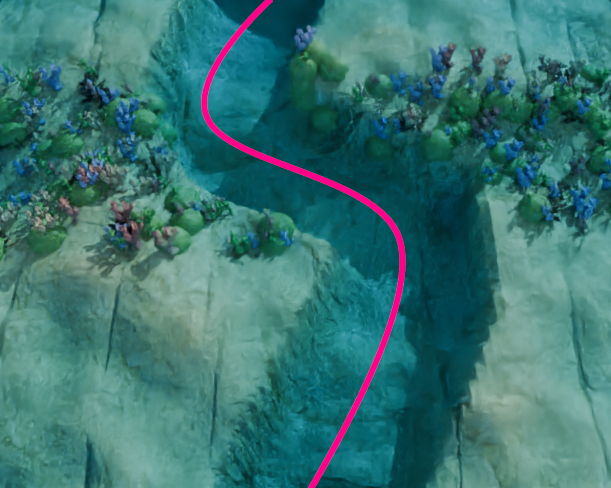
\includegraphics[width = 0.3 \linewidth]{Figures/Interactions/InteractionEdition1.png}
    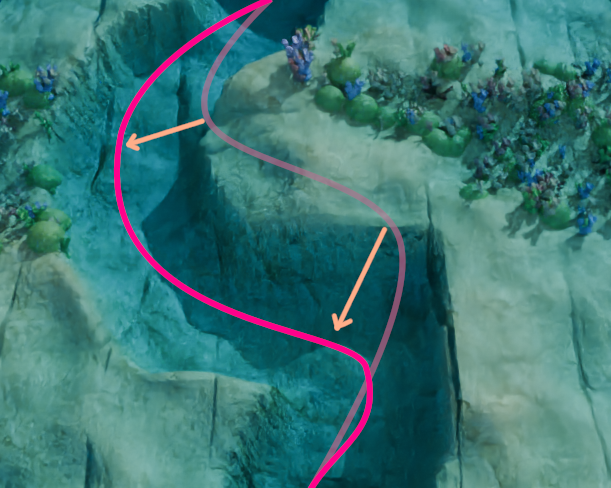
\includegraphics[width = 0.3 \linewidth]{Figures/Interactions/InteractionEdition2.png}
    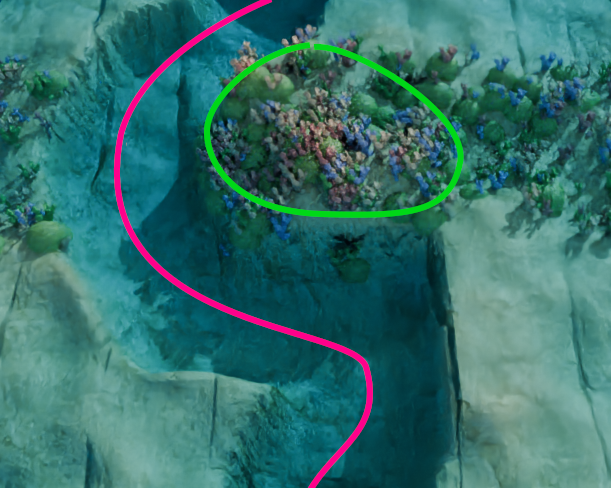
\includegraphics[width = 0.3 \linewidth]{Figures/Interactions/InteractionEdition3.png}
    \caption{Starting from a coral colony developed around a canyon (\textit{left}), the user edits the shape of the canyon, resulting in a different configuration of the scene, killing the corals that ends too deep in the water (\textit{center}) and the development and growth of new corals at the previous location of the canyon (\textit{right}). }
    \label{EnvironmentalObjects-fig:user-interaction}
\end{figure}

As long as a non-zero fitting function is defined in the terrain, new environmental objects can be forced by the user at any point of the simulation. 

% \subsubsection{Guiding the simulation}
Control over the region of the terrain that should be updated can be given by adjusting all fitting functions through a scalar field $\influence: \R^2 \to \R $ such that the fitting function $\fittingFuncObj(\p)$ of any new environmental object is evaluated as $\fittingFuncObj^*(\p) = \influence{\p} \fittingFuncObj(\p)$. This is especially useful in the planning of robotic simulations as we can first generate the overall shape of our terrain and secondly focus the generation process around the areas that may be visited by the robot, avoiding useless simulations and computer power. 
Figure~\ref{EnvironmentalObjects-fig:coral-colonization-scene} shows an example of colonization of the coral polyps that we limited manually into an annulus.
% Figure~\ref{EnvironmentalObjects-fig:focus-area-example} shows an example of colonization of the coral polyps that we limited manually.

% \begin{figure}
%     \centering
%     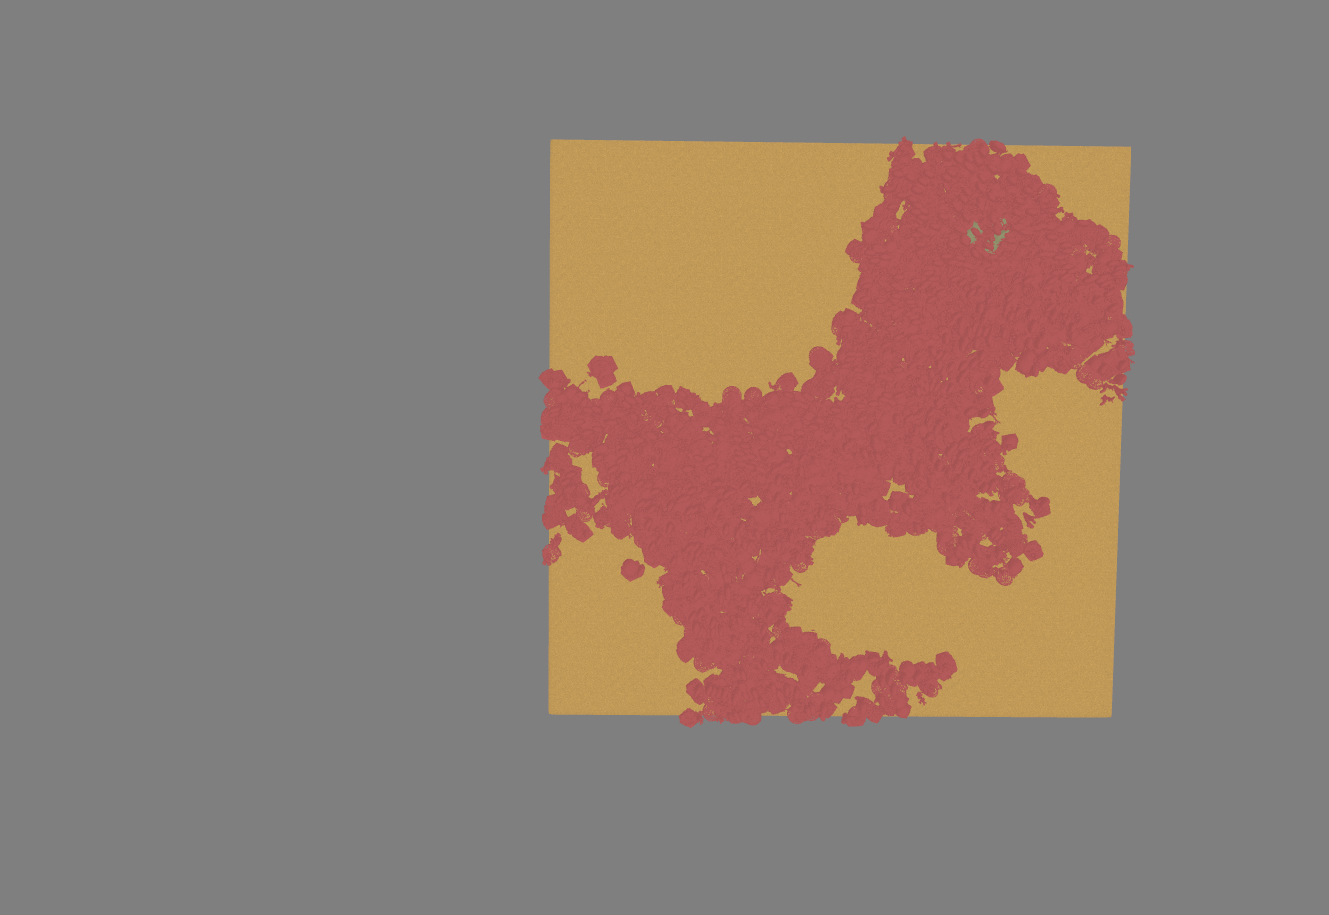
\includegraphics{Figures/UserControl/guidedGeneration1.png}
%     \caption{Controlling the generation area can produce a user-defined focused shape.}
%     \label{EnvironmentalObjects-fig:focus-area-example}
% \end{figure}

% - Changing the water currents \\
Our water current simulation is modeled as a simple vector field. As such, the user is able to interact with it at any moment of the simulation, allowing for the death of sensible environmental objects while it will guide the simulation into a new landscape. By modifying the water currents, the user also modifies the transport rate of materials at this position. The modification of currents is given as a stroke, a parametric curve $\curve$ for which we evaluate $\Delta \Wuser(\p)$ just as for curved environment objects (Section~\ref{EnvironmentObjects-sec:water-currents}).

\subsubsection{Geological events}
\label{EnvironmentObjects-sec:events}
A configuration file can define in advance the different events that should be triggered during the simulation. This can be useful to generate landscapes that are close to some existing locations. 
Multiple geological events can be triggered either as sudden or continuous environmental changes. These changes play a huge role in the morphology of landscapes.
We define events with a starting point and an ending point, such that at any time of the simulation we can compute the progress of the event as $\tEvent \in [0, 1]$.

Water level changes are important events that shape the underwater landscapes. As previously submerged environmental objects get elevated above water level, flora and fauna terrain elements dry and die. Deprived from the living part of the elements, everything is more affected by terrestrial erosion. By updating the value of the depth $\depth$ evaluated in the fitting functions, any environmental object that is sensible to the depth will be impacted automatically, that may be causing death (Figure~\ref{EnvironmentalObjects-fig:water-event}). The modification of the water level is defined as 
\begin{align*}
    \depth(\p) = \depth_0(\p) + \sum_{e \in \events} \Delta \depth_e \tEvent
\end{align*}
with $\Delta \depth_e$ the amount of water rising or lowering during an event. We assumed a linear evolution of the water level during an event. This allows to evaluate the depth at any point in space and in time.

\begin{figure}
    \centering
    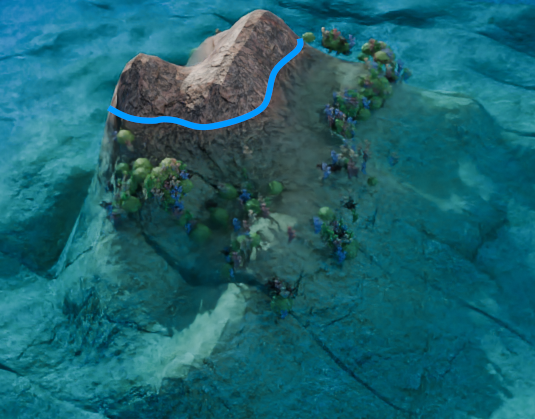
\includegraphics[width = 0.45 \linewidth]{Figures/Interactions/InteractionWater1.png}
    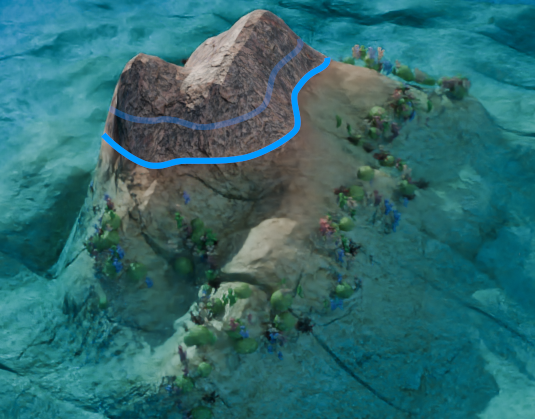
\includegraphics[width = 0.45 \linewidth]{Figures/Interactions/InteractionWater3.png}
    \caption{Lowering the water level by a few meters caused most of the coral objects to satisfy $\fittingFuncObj \leq 0$, causing their death. Since the water level (blue) decrease slowly, new coral objects spawn progressively at a lower altitude.}
    \label{EnvironmentalObjects-fig:water-event}
\end{figure}

Subsidence and uplift are the main geological events that create or destroy islands in the long term. These events are simulated as a simple factor on the height field of the generated terrain (Figure~\ref{EnvironmentalObjects-fig:subsidence-event}). Subsidence is not always uniform in the terrain. As such, the user can provide a position $\q$ at which the subsidence is the strongest, the amount of subsidence applied $\Delta \height_e$ and a standard deviation $\std$ for which we can then compute at any point in space and time of the simulation the height of the terrain
\begin{align*}
    \height(\p) = \height_0(\p) \cdot \sum_{e \in \events}{\frac{G(\norm{\p - \q})}{G(0)}} \Delta \height_e \tEvent 
\end{align*}
with $G(x)$ the Gaussian function
\begin{align*}
    G(x) = {\frac {1}{\std {\sqrt {2\pi }}}} \exp \left(-\frac {x^{2}}{2 \std ^{2}}\right)
\end{align*}

\begin{figure}
    \centering
    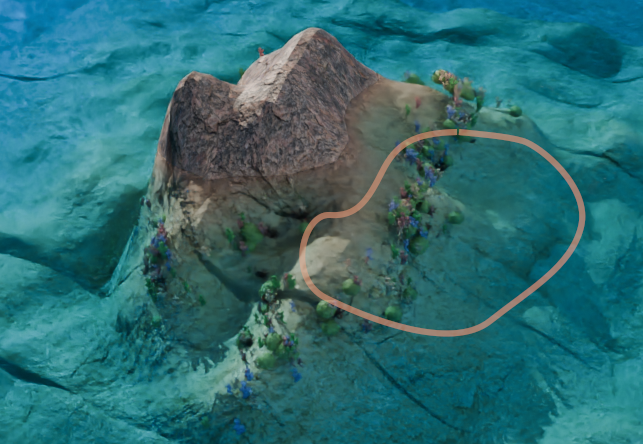
\includegraphics[width = 0.45 \linewidth]{Figures/Interactions/InteractionSubsidence1.png}
    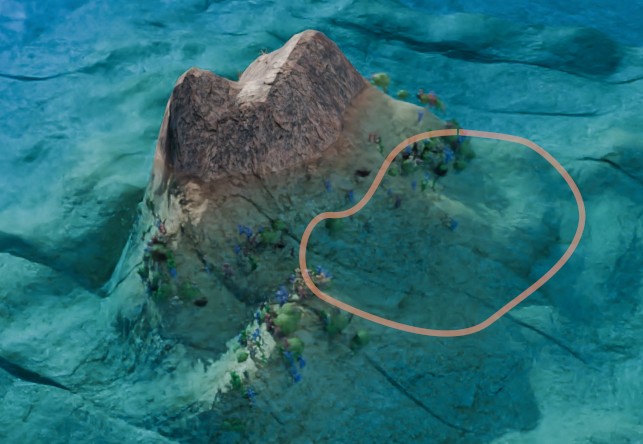
\includegraphics[width = 0.45 \linewidth]{Figures/Interactions/InteractionSubsidence2.png}
    \caption{Simulating subsidence on a part of the terrain (brown area) cause the depth value to change locally, resulting in the death of coral objects that find themselves too deep to survive. Here two subsidence events are triggered in parallel. }
    \label{EnvironmentalObjects-fig:subsidence-event}
\end{figure}

Storms are factors of the geomorphology of coral reefs \cite{VilaConcejo2016, Oron2023} and coasts \cite{Dominguez2005, Cowart2010}. Due to the extreme wind and wave velocities coasts are highly eroded in a short time period and the more fragile corals near the water surface are broken, possibly causing breaches in the reefs and spreading polyps in the currents direction. While there are many factors at play to understand the apparition of storms and the hydrodynamics affecting it, we simplified the model of storms to the user as a single epicenter $\q$ with a wind velocity $\windVelocity$ and a standard deviation $\std$ representing the spread around the epicenter (Figure~\ref{EnvironmentalObjects-fig:storm-event}). The computation of water currents are then computed as 
\begin{align*}
    \Wuser(\p) = \Wuser^*(\p) + \sum_{e \in \events | \tEvent \in [0, 1]} {\windVelocity \frac{G(\norm{\p - \q}}{G(0)}}
\end{align*}
In this case, we did not include the linear factor $\tEvent$ as storms are usually conserving a constant force for the time of the few weeks or months of their occurrence. 

\begin{figure}
    \centering
    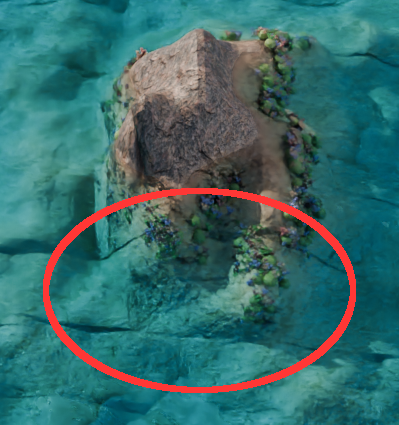
\includegraphics[width = 0.45 \linewidth]{Figures/Interactions/interactionStorm1.png}
    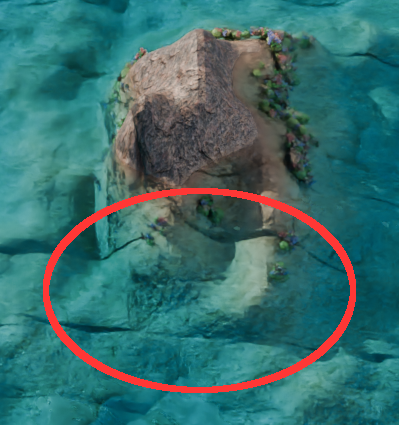
\includegraphics[width = 0.45 \linewidth]{Figures/Interactions/interactionStorm2.png}
    \caption{The result of a storm localized on one side of the island (red area) modifies the result of the evaluation of environmental objects around its epicenter for a short period of time. Most of the coral objects died from the event, except few environmental objects less sensible to water currents strength. }
    \label{EnvironmentalObjects-fig:storm-event}
\end{figure}

% Just as for the rise and lowering of water level, the heat is modeled as a simple value of the environment. For shallow areas (<100m) we assume a linear relation between depth and temperature, and a constant value for the terrestrial environment. As such, we can model a heat wave by a change of the environment values. Environmental objects who are sensible to temperature may die instantly. The modification of the temperature is defined as 
% \begin{align*}
%     \temperature(\p) = T_0(\p) + \sum_{e \in events} \Delta \temperature_e \tEvent + c \depth(\p)
% \end{align*}
with $\Delta \temperature_e$ the change of heat during an event, $\temperature_0$ the temperature at the water surface, and $c$ a very small factor.

The framework can easily be extended as the geological event system stays similar for all events. Including higher level simulations in the event system can be added, such as the simulation of tectonic activity, the use of fluid dynamics for tsunami events, the integration of human activity, ...

\section{Expert knowledge integration}
\label{EnvironmentObjects-sec:biology}
  The definition of the fitting functions of the environmental objects are inspired by the biological and geological factors that rule the evolution of underwater landscapes. The main factors are depth, light, water currents and biodiversity. External events have direct and indirect repercussions on the biodiversity of underwater environments. Coral islands are complex bio systems in which fauna, flora and geology are mixed together. 

\subsection{Environmental objects description}
\label{EnvironmentObjects-sec:represented-objects}
We have represented with environmental objects some geologic elements, animal elements and flora elements. The low island is most often raised in a circular shape as the process mainly appear around a hot spot under the ground. The evolution of an island into a coral island requires that the environmental conditions are sufficient for coral development: corals will grow slightly below the water surface as waves will break its growth and at a shallow depth (around 3m to 30m deep) in order for light to reach it. As coral grow and die, the skeleton is transformed into porous limestone, providing shelter to surrounding animals and reducing the impact of water erosion on the island. Corals drop polyps that are transported by the water flow and when they stick to a hard surface, as a rock or the reef itself, the coral may grow and colonize the area. As subsidence cause the island to lower, the living part of the coral reef keep growing toward light, which lead to a reef that is constantly close to the water level without reaching it due to wave erosion. The survival of reefs depends on the equilibrium between coral growth and and erosion. Eroded parts of the reef falling in the sheltered part of the reef accumulates, ending up by forming a lagoon. An island formed by a hot spot will inevitably subside in time, until it is completely flatten. As the coral reefs keep growing, only the lagoon remain, resulting in an atoll. \\
In this work we we integrate the biological and geological knowledge in the fitting functions of the environmental objects we want to generate. We represent the islands as regions that can be appearing with a uniform distribution. From the formulation of the region description \eqref{eq:internal-energy-equation}, we mostly create circular islands. The coral elements, environmental objects described as a single point, have a fitting function that take into account the depth of the ground, the amount of sand, fresh water and polyps in their environment, as well as the strength of water currents. Each coral species have different living conditions, but we reduced our work to soft coral which are sensible to water strength and stony corals that are more resistant to erosion. Reefs are formed as coral's skeleton are transformed into calcareous stone, describing then as an environmental object representing multiple others. 

\subsection{Simplifications}
\label{EnvironmentObjects-sec:simplifications}
The environmental factors simulated are greatly simplified as the real processes are in a very small time scale, that computer simulation are not able to simulate in interactive time. The use of environmental objects aim to represent a plausible results, while avoiding modeling the smaller scale events. Examples of simplifications are the geometry and material of each environmental object, which have an influence on the water currents through friction, the water currents represented as stationary flows, while the water flow dynamics are a complex system that may change completely at two different times of the day, the animal influence on the reefs that they transform by the ingestion and deposition of sediments, ...


\section{Results}
\label{EnvironmentObjects-sec:results}
Our method provides a way to generate scenes at different scales. We demonstrate this capacity with the generation of a large scene of an island (Figure~\ref{EnvironmentObjects-fig:teaser}) after what we focused the generation process in a canyon (Figure~\ref{EnvironmentalObjects-fig:canyon-scene}), then a small-scale visualization of coral colonies (Figure~\ref{EnvironmentalObjects-fig:coral-colonization-scene}).
In the examples, we rendered the environmental objects as a implicit tree or as individual meshes. The island, lagoons, reefs, canyons and sand ripples as implicit surfaces

% \subsection{Mid-scale}
% \label{EnvironmentObjects-sec:mid-scale}
A canyon scene can be generated using our method. The water flow is affected by the curve of the canyon such that the currents are oriented in the direction of the curve's tangent.In this example, we force the position of arches to be inside the canyon. The arches deposits a material "rock deposit", which is the main element of the fitting function of the Rock object. The "rock deposit" is slightly affected by water currents, but its mass make it highly affected by gravity. As such, rocks will spawn underneath arches. In reality, an arch is often created as part of a large coral boulder that sees the calcareous bottom part detached by the water currents, often resulting in an arch surrounded by big rocks and smaller rocks from the erosion of the first rocks.
As such, we define an environmental object "Arch" with a fitting function $\fittingFunc_{arch}(\p) = 5 - d(canyon - \p) * \norm{\Water(\p)}$, an environmental object "Rock" using $\fittingFunc_{rock}(\p) = \material_{rock\_deposit}(\p)$ and Pebble using $\fittingFunc_{pebble}(\p) = \material_{smaller\_rock\_deposit}(\p)$. Finally, sand ripples are simply described as curves appearing where there is a lot of sand available: $\fittingFunc_{ripple}(\p) = \material_{sand}(\p)$.
Following these simple rules, Figure~\ref{EnvironmentalObjects-fig:canyon-scene} shows the emergence of details in the scene. 

% \subsection{Small-scale}
% \label{EnvironmentObjects-sec:small-scale}
In this example we defined three different types of corals, coralA, coralB and coralC, to illustrate the possibility to model behaviours from the choice of fitting functions. Each of the coral types deposits a material "coral polyp" and "coral polyp A" ("coral polyp B" and "coral polyp C" respectively). By considering a fitting function that minimize the ratio $\frac{\text{coral polyp}}{\text{coral polyp A}}$, we can see an emergent behavior of the three types of coral fighting for the space colonization.
Figure~\ref{EnvironmentalObjects-fig:coral-colonization-scene} shows the result of this simulation at three different interations. At the border between two colonies, none of the colonies make progression due to the amount of coral polyp specific from the other colony.

\begin{figure*}
    \centering
    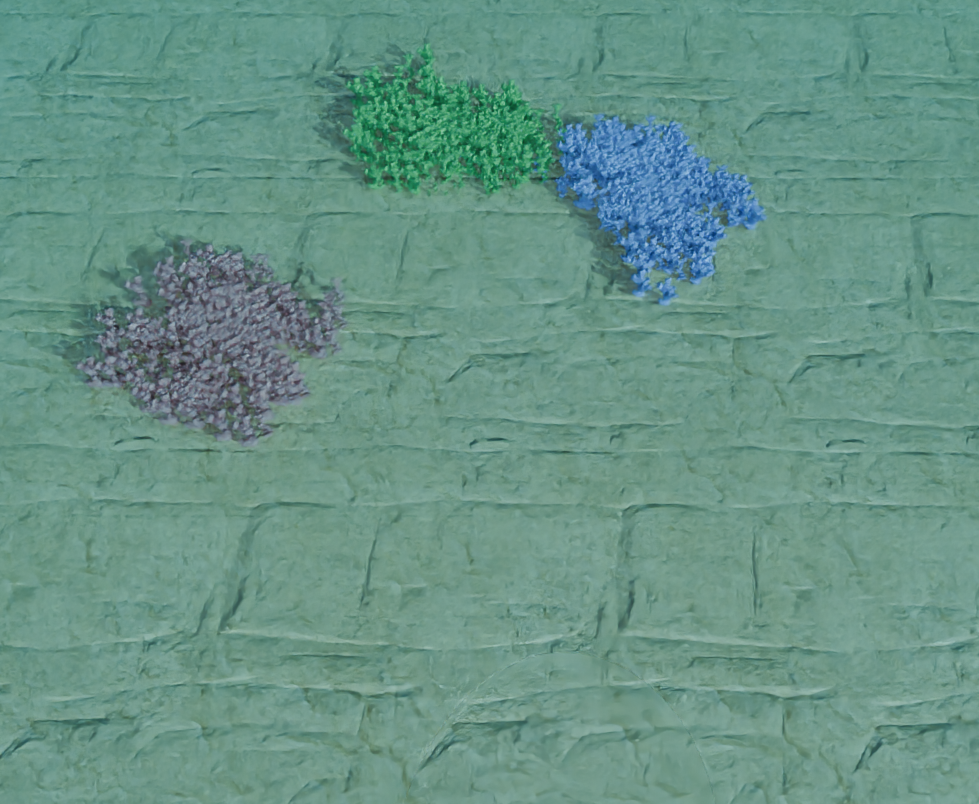
\includegraphics[width=0.245 \linewidth]{Figures/Colonization/col0.png}
    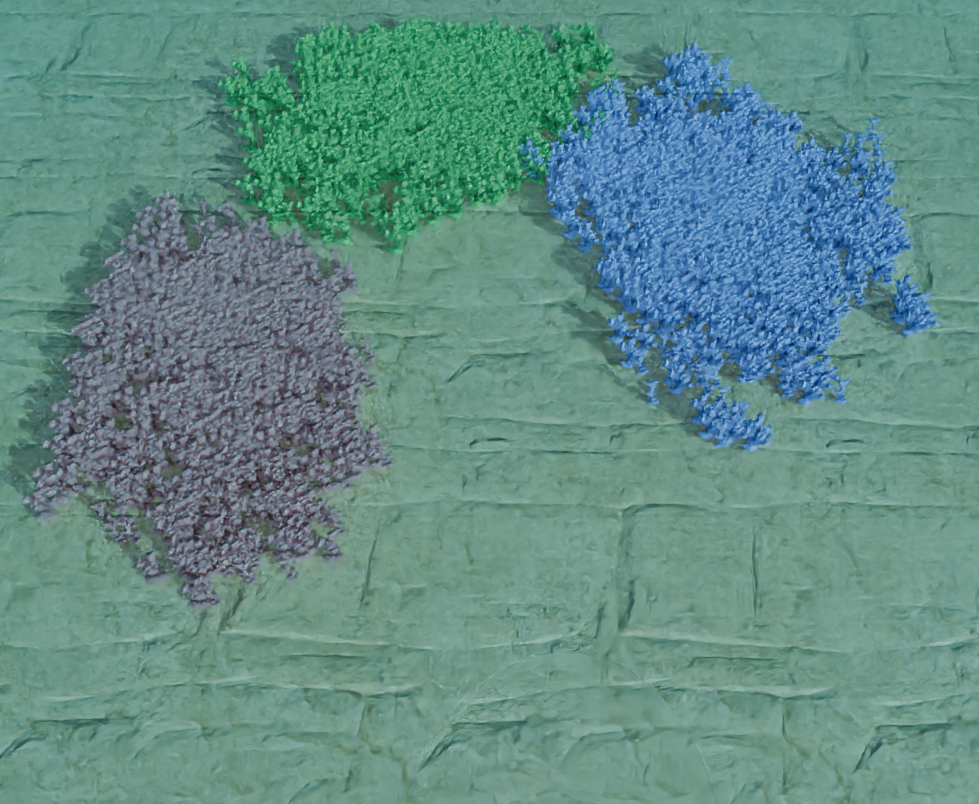
\includegraphics[width=0.245 \linewidth]{Figures/Colonization/col1.png}
    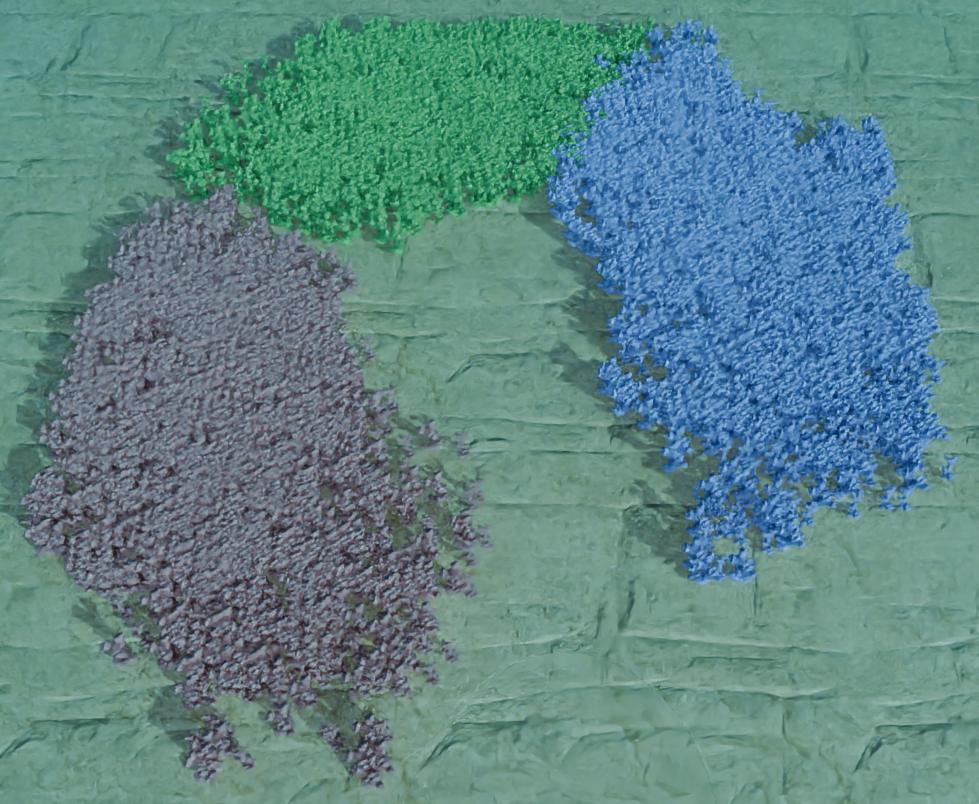
\includegraphics[width=0.245 \linewidth]{Figures/Colonization/col2.png}
    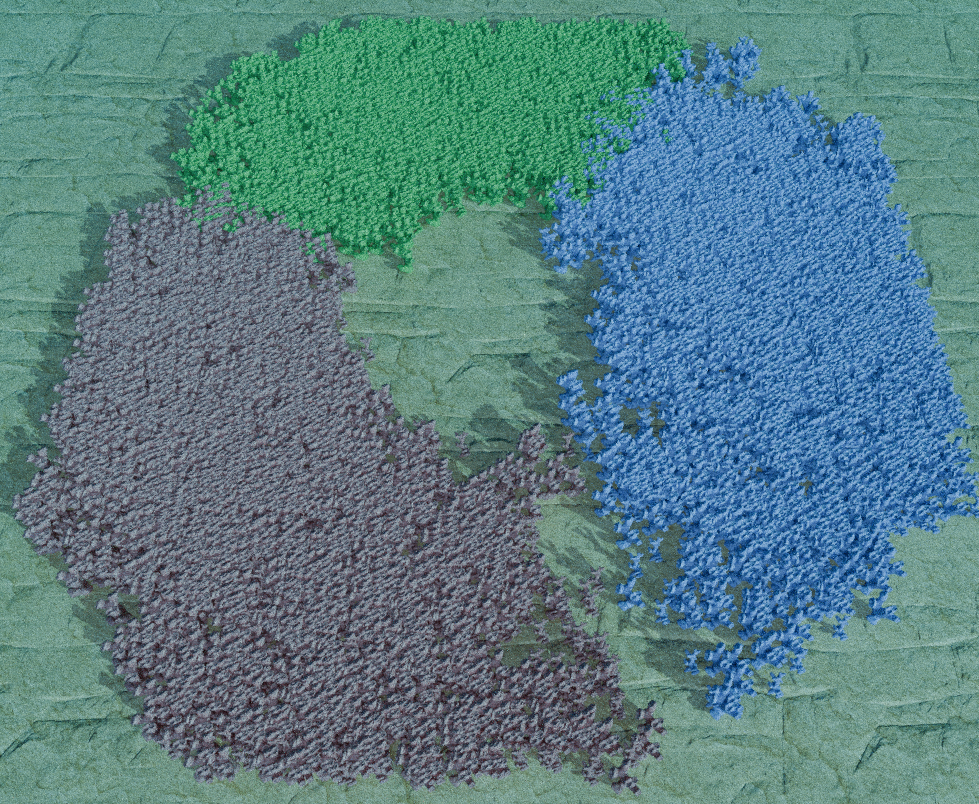
\includegraphics[width=0.245 \linewidth]{Figures/Colonization/col3.png}
    \caption{Three colonies of coral (red, blue, green) restricted to an annulus the middle section of the terrain fighting for the space.}
    \label{EnvironmentalObjects-fig:coral-colonization-scene}
\end{figure*}

\begin{figure*}
    \centering
    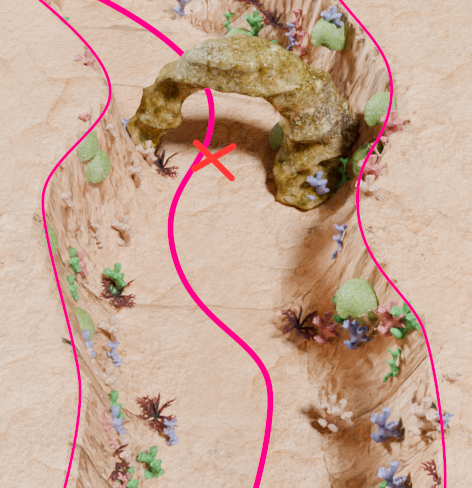
\includegraphics[width = 0.24 \linewidth]{Figures/Canyon/Canyon2.png}
    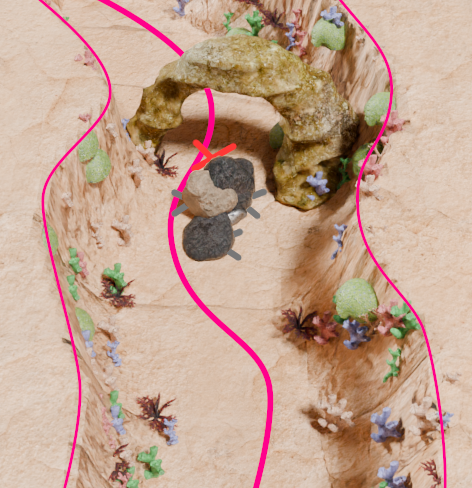
\includegraphics[width = 0.24 \linewidth]{Figures/Canyon/Canyon3.png}
    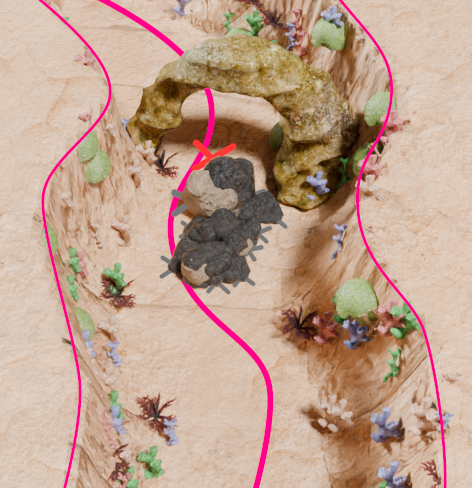
\includegraphics[width = 0.24 \linewidth]{Figures/Canyon/Canyon4.png}
    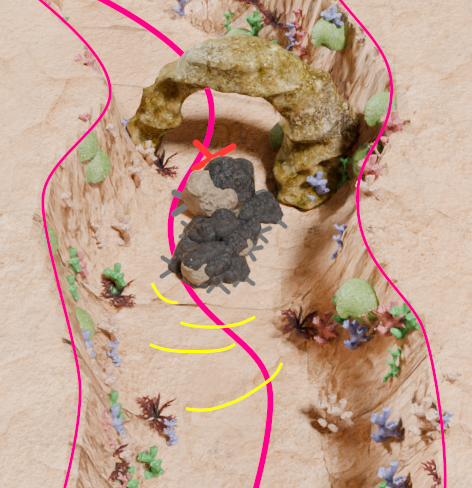
\includegraphics[width = 0.24 \linewidth]{Figures/Canyon/Canyon5.png}
    \caption{Evolution of a canyon scene at different iterations of the simulation. The apparition of an arch causes the spawning of rocks, pebbles, and finally some deposition of sand at the bottom of the canyon, spawning ripples. }
    \label{EnvironmentalObjects-fig:canyon-scene}
\end{figure*}



\section{Discussion}
\label{EnvironmentObjects-sec:discussion}
The proposed method aims to generate plausible landscapes using simplified versions of the evolution of an ecosystem and of the 3D representation. The biological realism of the result is highly correlated to the amount of simplification and assumptions, while the visual realism is completely dependent to the geometric functions used for the 3D modeling of the environmental objects. While proposing a flexible method that propose a generic approach for terrain generation, a close collaboration with fields experts and with graphists is needed to achieve optimal results.

Most simulation algorithm's quality depends on the size of the time step used, but with the introduction of a decay rate in the materials properties, we limit the influence of time steps by considering that steady-state are reachable. The material deposition and absorption on punctual environmental objects can be seen as a Dirac function $\dirac$ centered at their position resulting in the advantage that material displacement function can use the definition of the diffusion equation instead of the advection-diffusion-reaction equation. This equation allowing us to evaluate the state of the material $\material$ without intermediate steps, but this is not applicable with curve- and region-based environmental objects. 

\section{Conclusion}
\label{EnvironmentObjects-sec:conclusion}
We have proposed a method to generate terrains procedurally using sparse representations. This representation, the environmental objects, enables to introduce expert knowledge by the mean of the fitting functions that rule the environmental objects life cycle, but also to integrate the user in the loop during the generation process. We reduced the terrain resolution limitations by defining the environment objects as parametric elements. Thanks to the sparse representation based on single points, curves and regions, we allow for direct manipulation of the environmental objects of the scene by the user which, thanks to the environment steady state consideration, also enables to include these interactions in the automatic simulation process. \\
Integrating environmental properties in the fitting function of environmental objects allows the user to guide the generation through geological events. Our method enables each environmental object of the scene to influence the environment locally, reducing the need of computations while also retrieving environment values locally, which result in a parallelizable life-like simulation process. The genericity of the environment properties definitions should be sufficient for plausible generation of other landscape types as long as expert knowledge can be translated to environmental object's formalism.


We limited our work to the use of 2D scalar fields as they are more easily differentiable, interpretable and lighter than volumetric representations. However, future works include using 3D representations of the terrain and the environment to generate 3D terrains, including cavities, sub-terrestrial areas and the interior of coral structures. 
% The different possibilities to explore for this would be: the use of 3D particles to represent the state of the materials in the environment, or voxel grids or flatten representation of the terrain's surface (but would not allow a different morphological shape than the height field...).

\def\url#1{} % This line actually remove the "URL" link from the references


\begin{figure*}
    \centering
    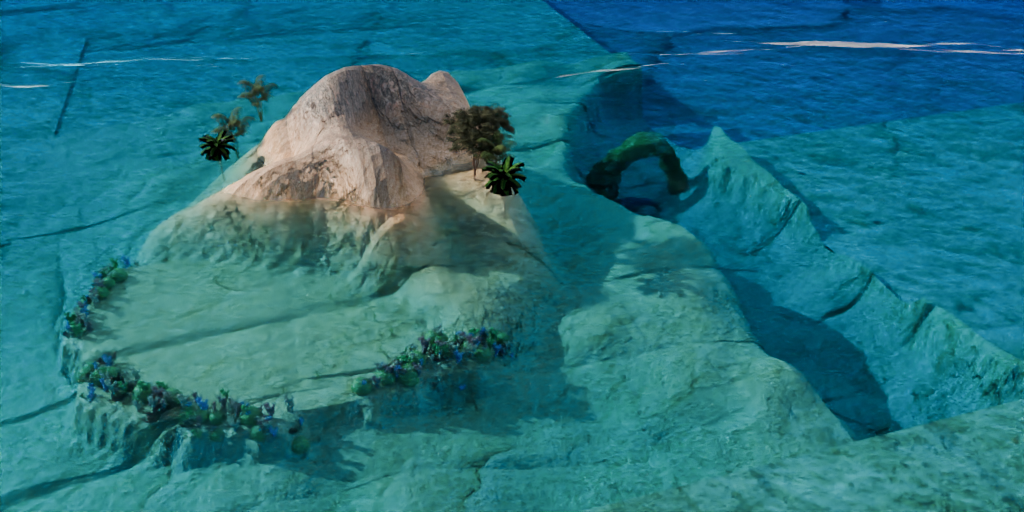
\includegraphics{Figures/CoralIsland/multiScene1 v2 final 1.png}
    \caption{A simple coral island is generated using an island, a lagoon, reefs coral polyps, beaches, trees and algae environmental objects. Trees appear on beaches and algae grow in the lagoon's sand. }
    \label{EnvironmentalObjects-fig:coral-island-scene}
\end{figure*}

% bibtex
%\bibliographystyle{eg-alpha-doi}
%\bibliography{references_terrain}

% biblatex with biber
% \printbibliography

%\end{document}